\section{Statistical Analysis System (SAS)} \label{section: SAS}
SAS, or Statistical Analysis System, is a software suite that has been used for advanced analytics, business intelligence, data management, and predictive analytics since it was first released in 1976. Developed by the SAS Institute, it offers a range of statistical and data analysis tools, which are suitable for many applications including data mining, forecasting, econometrics, quality control, and statistical analysis.

The software provides a user-friendly graphical interface for data analysis and reporting, as well as a powerful programming language that allows users to customize their analysis and automate repetitive tasks. Its ability to handle large and complex datasets and perform advanced statistical analyses make it popular in various industries, including finance, healthcare, government, and academia. SAS is widely used for purposes such as fraud detection, risk management, clinical research, and marketing analysis, and is a popular choice among data scientists and statisticians. 

SAS offers multiple product\href{https://www.sas.com/en_us/software/all-products.html#all-products-a-z}{\textbf{ suites}}. The SAS Enterprise Suite is a collection of SAS products designed for enterprise-level data management and analysis, such as SAS 9.4, SAS Visual Analytics, SAS Data Integration Studio, SAS Data Management, etc. The SAS Platform provides two engines for managing foundational capabilities such as distributed processing, security, administration, program development and execution, resource management, user interfaces, cloud integration, operating systems and third-party software. These engines are \href{https://documentation.sas.com/doc/en/pgmsascdc/9.4_3.5/whatsnew/n17cszme3e52b4n1ooe3710fnuec.htm#:~:text=Initial%20Release%20of%20SAS%209.4,-The%20initial%20release&text=For%20SAS%20administrators%2C%20SAS%209.4,more%20complete%20data%20management%20solution.}{\textbf{SAS 9.4}} and \href{https://documentation.sas.com/doc/en/pgmsascdc/9.4_3.5/pgmsasgswlcm/home.htm}{\textbf{SAS Visual Analytics}}. 

\subsection{SAS 9.4}
\href{https://documentation.sas.com/doc/en/pgmsascdc/9.4_3.5/whatsnew/n17cszme3e52b4n1ooe3710fnuec.htm#:~:text=For%20SAS%20administrators%2C%20SAS%209.4,more%20complete%20data%20management%20solution.}{SAS 9.4} is a software suite that provides tools for data management, statistical analysis, business intelligence, and predictive modeling. SAS 9.4 can handle large datasets and complex analyses by using a wide range of built-in functions and procedures that can save time and effort when working with data. 

For example, a pharmaceutical company might use SAS 9.4 to analyze clinical trial data to determine the efficacy and safety of a new drug. A bank might use SAS 9.4 to perform risk analysis on its loan portfolio. A retail company might use SAS 9.4 to analyze customer data to better understand buying patterns and preferences.

SAS 9.4 is composed of several modules that provide a wide range of functionalities:
\begin{itemize}
    \item Base SAS - Provides the basic programming language, data access, and management capabilities of SAS.
    \item SAS/STAT - Provides a comprehensive set of statistical analysis procedures for data exploration and modeling.
    \item SAS/GRAPH - Provides a set of tools for creating high-quality graphical output from SAS data.
    \item SAS/ETS - Provides a set of time series analysis and forecasting procedures.
    \item SAS/IML - Provides an interactive matrix language for matrix manipulation, data analysis, and numerical optimization.
    \item SAS/ACCESS - Provides connectivity to data sources such as relational databases and spreadsheets.
    \item SAS Enterprise Guide - Provides a graphical user interface (GUI) for SAS programming, data management, and reporting.
\end{itemize}

\subsection{SAS Data Management Advanced (SAS DMA)}
SAS DMA is a part of SAS 9.4 as a software suite to support data management and analytics. SAS DMA is not a separate module or component in SAS 9.4. Instead, it is a set of data management tools and techniques that are included in various SAS modules, such as Base SAS, SAS/ACCESS, SAS Enterprise Guide, etc. It comprises three components: mid-tier, metadata, and compute.

The mid-tier component provides a web-based interface for accessing SAS services and applications. It includes a web server and the SAS Web Application Server (WAS) component, which acts as a middleware layer between the SAS software and the user interface. Users can access the SAS mid-tier web interface using a web browser to interact with the SAS services and applications deployed on the SAS compute component.

The metadata component serves as a central repository for metadata, such as information about SAS servers, libraries, and user accounts. Other SAS components use it to manage and share metadata across the SAS environment. SAS administrators typically manage the SAS metadata component, although users may interact with it indirectly through the SAS mid-tier interface.

The compute component provides the computational resources needed to run SAS applications and services. It includes the SAS server software, which runs SAS programs and manages data access, processing, and storage. The SAS compute component may be deployed on a separate server or on the same server as the other SAS DMA components, depending on the specific deployment architecture.

\subsection{SAS Visual Analytics (SAS Viya)}
SAS Viya, or SAS Visual Analytics, is a cloud-enabled, in-memory analytics engine that provides elastic, scalable, and fault-tolerant processing for advanced data analytics, data processing, and machine learning for enterprise environments. SAS Viya includes a variety of tools such as SAS Visual Analytics, SAS Visual Statistics, SAS Data Mining, and SAS Machine Learning. When performing analytics on large datasets, SAS Viya uses a distributed in-memory processing engine called \href{https://documentation.sas.com/doc/en/calcdc/3.3/calserverscas/n05000viyaservers000000admin.htm}{\textbf{CAS}}.

\subsection{Cloud Analytics Services (CAS)}
Cloud Analytics Services (CAS) is the in-memory analytics engine SAS Viya uses for both on-premise as well as cloud-service environments (e.g., AWS, Azure, GCP). CAS uses a combination of hardware and software where data management and analytics take place on either a single-machine or as a distributed server across multiple machines. In either single or distributed deployment, each machine (host, node, etc) will be assigned one of three roles: CAS Controller, CAS Backup Controller, CAS Worker.

\textbf{Analogy}
\\
In a restaurant kitchen, there exists three primary chefs. They are the (1) executive chef, (2) sous chef, and (3) station chef(s). The executive chef's primary role is to manage the kitchen and its staff whilst doing very little cooking. The sous chef's primary role is to be the right-hand to the executive chef, ready to manage the kitchen, share, or take over the responsibility of the executive chef at a moments notice. The station chef(s) merely wait for instructions from the executive chef, then executes the job they are given. 

This is the relationship of each CAS node with each other:
\begin{itemize}
    \item The CAS Controller is the executive chef managing the kitchen and its staff, delegating work.
    \item The CAS Backup Controller is the sous chef ready to take over the responsibility of the executive chef. 
    \item The CAS Worker(s) are the station chefs cooking what they are assigned to by the executive chef. 
\end{itemize}

\subsubsection{Role 1: CAS Controller}
Controller is the first role that can be assigned to a host for SAS Cloud Analytic Services. For both server architectures, single-machine and distributed, one machine must be designated as the Controller. The role of the Controller is to parse out work to each Worker host available. In other words, the Controller manages and controls the overall operation of the CAS environment. As the master node, the Controller is responsible for distributing workload among available CAS Workers, managing user sessions, and providing a secure environment for data retrieval and data storage. 

In a single-machine environment, the CAS Controller and CAS Worker roles can be performed by different processes or threads within the same operating system instance. However, we are not limited to this deployment method as it is also possible to have the CAS Controller and CAS Worker(s) virtually separated (on the same hardware) to increase the scalability of the deployment. The configuration of your architecture depends on what you need out of CAS.  

In a distributed environment, the CAS Controller is responsible for managing and controlling the CAS environment whilst the actual data processing and data analytics are performed by the CAS Worker(s).
%insert diagram%

\subsubsection{Role 2: CAS Backup Controller}
Backup Controller is the second role that can be assigned to a host for SAS Cloud Analytic Services. Although optional, the CAS Backup Controller is highly recommended in a distributed server environment. The role of the CAS Backup Controller is to act as a standby or hot-backup for the primary CAS Controller in case of a failure. Its primary purpose is to ensure that the system can continue to function in the event of a failure of the primary controller. The Backup Controller is typically set to passively monitor the primary controller for any signs of failure, such as a loss of connectivity or failure to respond to heartbeat messages. It does not actively participate in task scheduling or job execution while the primary controller is running normally. 

If the primary CAS Controller fails, the Backup Controller will take over as the primary controller and assume responsibility for managing the CAS worker nodes and scheduling tasks. In this scenario, the CAS worker nodes will send their status updates and job results to the Backup Controller instead of the failed primary controller.\footnote{If the main CAS Controller fails, how does each CAS Worker respond to the Backup Controller with their completed jobs?}

In some systems, the Backup Controller can also be given jobs to execute as a CAS worker node. This can help to improve the system's overall performance by increasing the number of available processing resources. In this scenario, the Backup Controller can perform both the role of a CAS Controller and a CAS worker node.\footnote{Can the CAS Backup Controller be assigned work as well as passively monitor the main CAS Controller?}

%insert diagram%

\subsubsection{Role 3: CAS Workers}
Worker is the third role that can be assigned to a host for SAS Cloud Analytic Services. The CAS Worker is responsible for performing data processes and data analytics sent from the CAS Controller. For example, CAS Workers can perform data manipulations, transformations or computations on large/complex datasets. These computations are but not limited to: statistical analysis, machine learning models, text analysis, time series analysis, optimization, etc. Workers execute these computations using data stored on disk, in-memory, or in a distributed file system. 

In a distributed environment, one host will be assigned as your controller and any additional hosts are considered workers (optional CAS Backup Controller). Workers increase the overall computing power of your distributed-server and provides a solution for a scalable (up/down), distributed, and fault-tolerant environment for data storage and data analysis because the worker manages the storage of data/metadata across multiple nodes. The amount of CAS Workers needed to create an optimized distributed environment is highly dependant on data size, computation type, and workload.  
%insert diagram%

We can create two types of CAS configurations: a single-machine environment using symmetric multiprocessing \href{https://documentation.sas.com/doc/en/calcdc/3.3/calserverscas/n05000viyaservers000000admin.htm}{\textbf{(SMP)}}, or distributed server environment using massively parallel processing \href{https://documentation.sas.com/doc/en/calcdc/3.3/calserverscas/n05000viyaservers000000admin.htm}{\textbf{{(MPP)}}}.

\subsubsection{Symmetric Multiprocessing (SMP)}
The Symmetric multiprocessing (SMP) architecture is used when you want to run CAS on a single server or virtual machine (VM) with multiple CPU cores. This is called shared-memory architecture because all the CPUs share the same memory. When a job is submitted to CAS in an SMP architecture, it is processed by the worker node(s) in parallel using the shared memory. The results are returned to the controller node, which sends them back to the user.

A typical SMP architecture for CAS might consist of a single VM that serves as both the controller and worker node. The number of VMs required will depend on the size of your data and the processing requirements of your workload. For example, if you have a large dataset or complex analytical workloads, you might deploy CAS on a VM with 8 or 16 CPU cores.

Some examples of use cases for CAS on an SMP architecture include:

\begin{itemize}
    \item Exploratory data analysis
    \item Statistical modeling and regression analysis
    \item Predictive analytics
    \item Machine learning and deep learning
\end{itemize}

\begin{figure}[H]
    \centering
    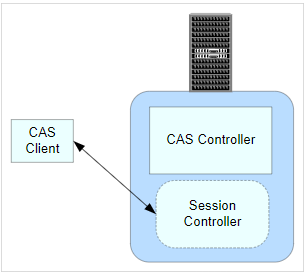
\includegraphics[scale = 0.8]{images/smp_server.png}
    \caption{Single-machine CAS Server \textcolor{red}{(STOLEN EXAMPLE)} }
    \label{SMP Achitecture}
\end{figure}

\subsubsection{Massively Parallel Processing (MPP)}
The Massively Parallel Processing (MPP) architecture is used when you want to run CAS on a cluster of multiple servers or VMs. This is called distributed-memory architecture because the data is partitioned and stored across multiple servers or nodes. When a job is submitted to CAS in an MPP architecture, it is distributed across the worker nodes in parallel. Each worker node processes its own subset of the data and returns the results to the controller node. The controller node then aggregates the results from all worker nodes and sends them back to the user.

A typical MPP architecture for CAS might consist of multiple VMs or servers, with some dedicated as controller nodes and others as worker nodes. The number of VMs or servers required will depend on the size of your data and the processing requirements of your workload. For example, you might choose to deploy CAS on a cluster of 10 or more VMs or servers to handle large-scale data processing tasks.

Some examples of use cases for CAS on an MPP architecture include:
\begin{itemize}
    \item Big data processing and analysis
    \item High-performance computing
    \item Large-scale machine learning and deep learning
    \item High-throughput data processing, such as in genomics or drug discovery
\end{itemize}

\begin{figure}[H]
    \centering
    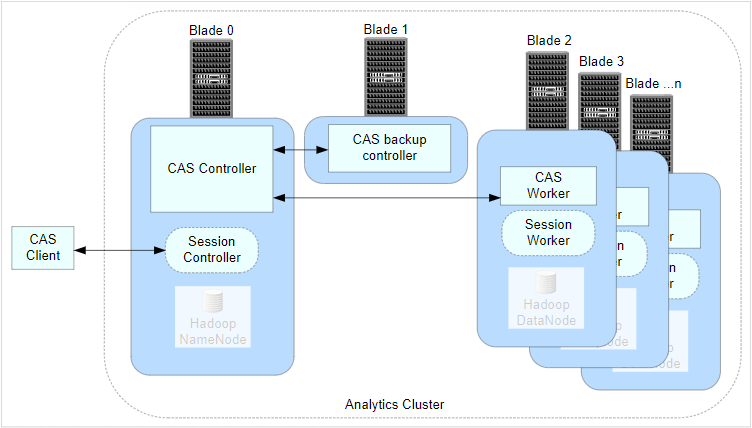
\includegraphics[scale = 0.70]{images/mpp_server.png}
    \caption{Distributed CAS Server \textcolor{red}{(STOLEN EXAMPLE)} }
    \label{MMP Architecture}
\end{figure}

